\subsection{Stokes flow}\label{sec:stokes}
The problem consists of determining velocity field $(u,v)$ and pressure $p$ in case of a manufactured solution with prescribed body forces such as
\begin{eqnarray}
b_1&=&(12-24y)x^4+(-24+48y)x^3+(-48y+72y^2-48y^3+12)x^2+\nonumber \\
&&+(-2+24y-72y^2+48y^3)x+1-4y+12y^2-8y^3\nonumber \\
b_2&=&(8-48y+48y^2)x^3+(-12+72y-72y^2)x^2+(4-24y+48y^2-48y^3+\nonumber \\
&&+24y^4)x-12y^2+24y^3-12y^4\nonumber
\end{eqnarray}
for which the exact solution is:
\begin{eqnarray}
u(x,y)&=&x^2(1-x)^2(2y-6y^2+4y^3)\nonumber \\
v(x,y)&=&-y^2(1-y)^2(2x-6x^2+4x^3)\nonumber \\
p(x,y)&=&x(1-x)-\frac{1}{6}\nonumber
\end{eqnarray}
\begin{figure}[h!]
\centering
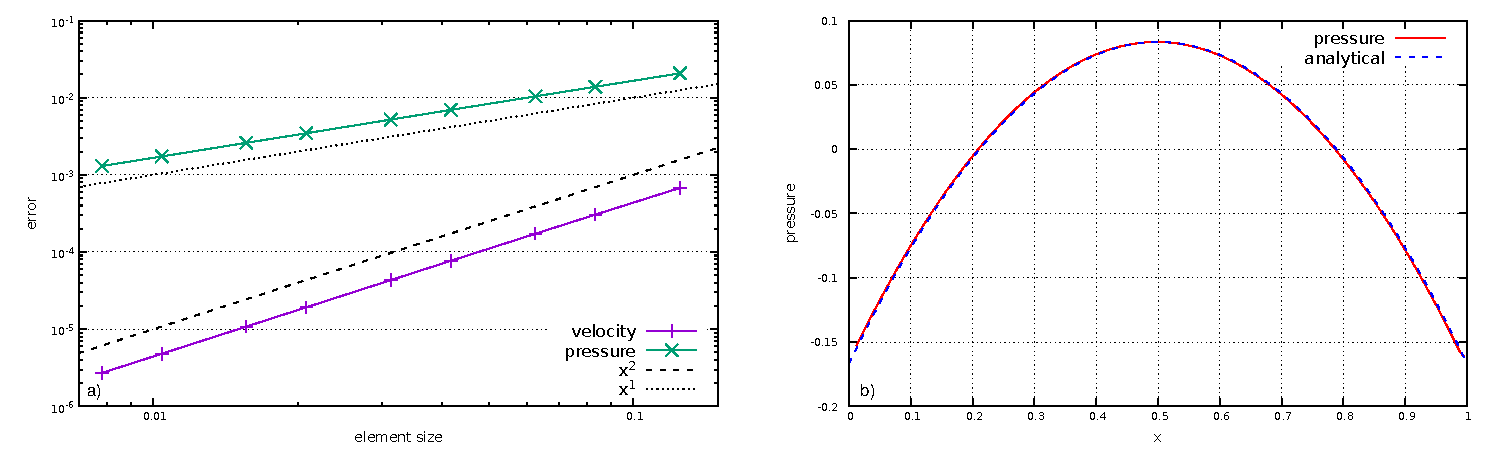
\includegraphics[width=13.5cm]{./Figures/errors.pdf}
\caption{Velocity and pressure error for the Stokes flow experiment between generated and analytical solution as a function of element size (panel a),
and comparison between smoothed pressure and analytical solution as function of $x$ coordinate for a grid resolution of $128\times128$ elements (panel b).}
\label{fig:errors}
\end{figure}
The domain is a unit square a constant viscosity ($\eta=1$) and the penalty parameter is set to $\lambda=10^7$. Velocity boundary conditions are set to no slip
$(\bm{v}=\bm{0})$ on all boundaries. The problem is performed for different grid resolution between $8\times8$ and $1024\times1024$ elements.
The errors between the analytical solution and the numerical prediction of the pressure and the velocity field are calculated by means of Eqs. \ref{errp} and \ref{errv}, respectively.
Fig. \ref{fig:errors}a shows that both velocity and pressure field converge to the exact solution with the decrease of the element size, following the
theoretical convergence rate. The convergence of pressure, in contrast with the observation by \citet{Donea2003} for $Q_1 \times P_0$ elements, indicate the
effectiveness of the smoothing procedure.
\begin{figure}[h!]
\centering
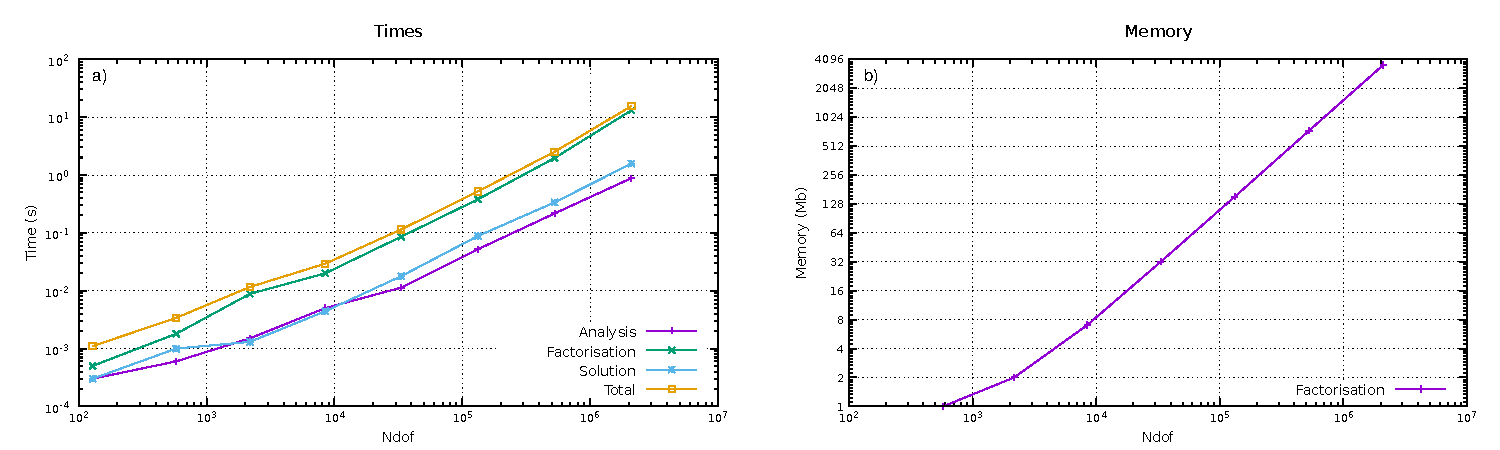
\includegraphics[width=13.5cm]{./Figures/MUMPS.pdf}
\caption{Analysis, factorisation, solution and total solve times (panel a) and factorisation memory usage (panel b) as a function of the total number
of degrees of freedom for the Stokes flow experiment.}
\label{fig:MUMPS}
\end{figure}
Smoothed pressure field for grid resolution of $128\times128$ elements is shown in Fig. \ref{fig:errors}b (continuous
red line), in comparison with the analytical solution (dashed blue line). Solve times and memory usage needed to generate the solution are shown in
Fig. \ref{fig:MUMPS}. All data can be found at \url{https://github.com/aleregorda/Benchmarks/tree/main/Solver/Stokes_Flow}.